\documentclass{standalone}
\usepackage{tikz}
\usetikzlibrary{fit}
\usepackage[dvipsnames]{xcolor}
\usetikzlibrary{shapes.geometric}
\newcommand\x{3.4}
\begin{document}
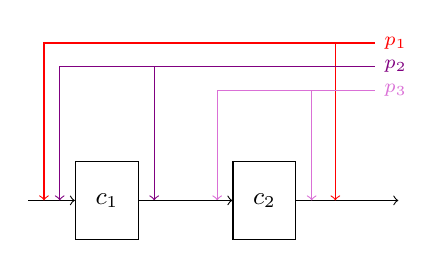
\begin{tikzpicture}[square/.style={regular polygon,regular polygon sides=4}, box/.style = {draw,red, dashed, inner sep=10pt,rounded corners=5pt}]
    \node at (0,0) [rectangle, minimum width = 0.8cm, minimum height = 1cm, draw] (o1) {\small $c_1$};
    \node at (2,0) [rectangle, minimum width = 0.8cm, minimum height = 1cm, draw] (o2) {\small $c_2$};

    \draw[->] (-1,0) -- (o1.west);
    \draw[->] (o2.east) -- (\x + 0.3, 0);

    %Probe 1
    \draw[->, red] (\x, 2) node[right] {\scriptsize $p_1$} -- (-0.8, 2) -- (-0.8, 0) ;
    \draw[->, red] (2.9, 2) -- (2.9, 0);

    %Probe 2
    \draw[->, violet] (\x, 1.7) node[right] {\scriptsize$p_2$} -- (-0.6, 1.7) -- (-0.6, 0);
    \draw[->, violet] (0.6, 1.7) -- (0.6, 0);
    %Probe 3
    \draw[->, Orchid] (\x, 1.4) node[right] {\scriptsize $p_3$} -- (1.4, 1.4) -- (1.4, 0);
    \draw[->, Orchid] (2.6, 1.4) -- (2.6, 0);

    \draw[->] (o1.east) -- (o2.west);

    \iffalse
\node at (0, 0) [circle, minimum size = 0.7cm, draw] (o1) {\small $o_1$};
    \node at (-1, 0) [square, draw] (s_1) {};
    \node at (1, 0) [square, draw] (e_1) {};
    \node at (2, 0) [circle, draw] (o2) {\small $o_2$};
    \node at (3, 0) [square, draw] (e_2) {};

    \draw (s_1.east) -- (o1.west);
    \draw (o1.east) -- (e_1.west);
    \draw (e_1.east) -- (o2.west);
    \draw (o2.east) -- (e_2.west);

    \node[label={\small probe}, box, fit=(s_1)(e_2)] {};
\fi
\end{tikzpicture}
\end{document}

